\documentclass{article}
\usepackage[utf8]{inputenc}
\usepackage{hyperref}
\usepackage{amsmath}
\usepackage{bera}
\usepackage{listings}
\usepackage{xcolor}
\usepackage{graphicx}
\usepackage{subcaption}
\usepackage{placeins}
\usepackage[paper=a4paper,margin=1.25in]{geometry}
\usepackage{bm}

\title{Comparing BLP, MIQP, and a Genetic Algorithm}
\author{Ryan Benasutti}
\date{\today}

\newcommand{\code}{\texttt}

\begin{document}

\maketitle

The arm being optimized,
\begin{figure}[h]
    \centering
    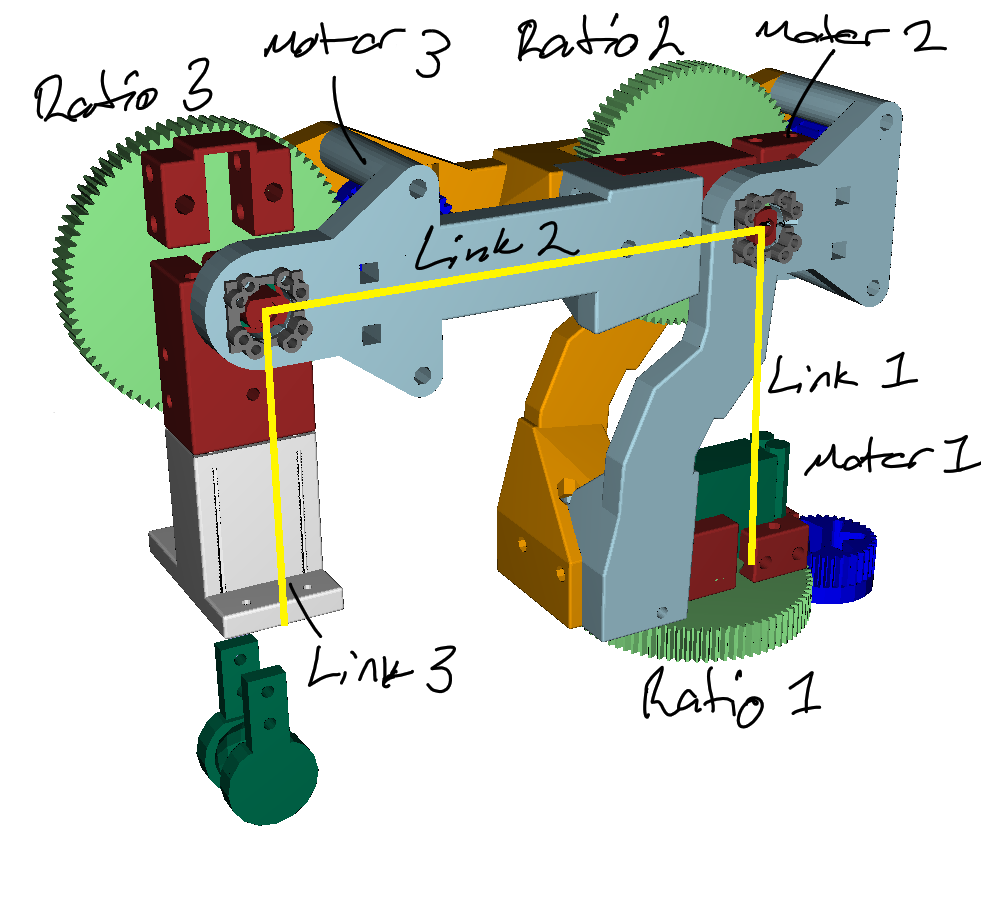
\includegraphics[scale=0.3]{annotated-arm.png}
    \caption{RBE 3001 3DOF Arm}
    \label{fig:annotated_arn}
\end{figure}

\FloatBarrier{}
\section{MIQP}

\FloatBarrier{}
\subsection{Feature Matrix}

The feature matrix of a motor module is given by
\begin{equation}
    F_m =
    \begin{bmatrix}
        \frac{\tau^{(1)}}{G^{(1)}} & & \frac{\tau^{(N)}}{G^{(N)}} \\[6pt]
        \omega^{(1)} G^{(1)} & & \omega^{(N)} G^{(N)} \\[6pt]
        P^{(1)} & \cdots & P^{(N)} \\[6pt]
        M^{(1)} & & M^{(N)} \\[6pt]
        G^{(1)} & & G^{(N)}
    \end{bmatrix}
\end{equation}

where $\tau^{(i)}$ is the stall torque in Newton-meters for motor $i$,
$\omega^{(i)}$ is the free speed in radians per second for motor $i$, $P^{(i)}$
is the price of motor $i$ in USD, $M^{(i)}$ is the mass in kilograms of motor
$i$, and $G^{(i)}$ is the gear ratio on motor $i$.

\FloatBarrier{}
\subsection{Variables}

$\tau_j$ denotes the $\tau$ of slot $j$, and $\omega_j$ denotes the $\omega$ of
slot $j$. $\tau_j$ and $\omega_j$ are implemented using a binary vector for
each slot $j$.

\FloatBarrier{}
\subsection{Constraints}

$V$ is the tip velocity, $F$ is the tip force, and $R_j$ is the r parameter of
link $j$. The arm is mounted $90 \deg$ off vertical.

\begin{equation}
    \tau_{1} \geq F(R_1 + R_2 + R_3) + G (M_2 R_1 + M_3 (R_1 + R_2))
\end{equation}

\begin{equation}
    \tau_{2} \geq F(R_2 + R_3) + M_3 G R_2
\end{equation}

\begin{equation}
    \tau_{3} \geq F R_3
\end{equation}

\begin{equation}
    \omega_{1} (R_1 + R_2 + R_3)\geq V
\end{equation}

\begin{equation}
    \omega_{2} (R_2 + R_3) \geq V
\end{equation}

\begin{equation}
    \omega_{3} R_3 \geq V
\end{equation}

\begin{equation}
    R_1 + R_2 + R_3 = 0.4
\end{equation}

\FloatBarrier{}
\subsection{Results}

MIQP took $0.03$ seconds to solve and found: \\
\texttt{
    Optimal objective: 40.89 \\
    Optimal motors: \\
    Motor("vexMotor-393", 1.637, 10.471, 14.99, 0.0945), ratio=0.3333333333333333, link1=68.0, link2=195.0, link3=137.0 \\
    Motor("stepperMotor-GenericNEMA14", 0.098, 139.626, 12.95, 0.12), ratio=0.05263157894736842, link1=68.0, link2=195.0, link3=137.0 \\
    Motor("stepperMotor-GenericNEMA14", 0.098, 139.626, 12.95, 0.12), ratio=0.05263157894736842, link1=68.0, link2=195.0, link3=137.0
}

\FloatBarrier{}
\section{BLP}

\FloatBarrier{}
\subsection{Feature Matrix}

The feature matrix of a motor module is given by
\begin{equation}
    F_m =
    \begin{bmatrix}
        \frac{\tau^{(1)}}{G^{(1)}} & & \frac{\tau^{(N)}}{G^{(N)}} \\[6pt]
        \omega^{(1)} G^{(1)} & & \omega^{(N)} G^{(N)} \\[6pt]
        P^{(1)} & & P^{(N)} \\[6pt]
        M^{(1)} & & M^{(N)} \\[6pt]
        G^{(1)} & & G^{(N)} \\[6pt]
        \ln(\omega^{(1)} G^{(1)}) & & \ln(\omega^{(N)} G^{(N)}) \\[6pt]
        R_1 & & R_1 \\[6pt]
        R_2 & \cdots & R_2 \\[6pt]
        R_3 & & R_3 \\[6pt]
        \ln(R_1) & & \ln(R_1) \\[6pt]
        \ln(R_2) & & \ln(R_2) \\[6pt]
        \ln(R_3) & & \ln(R_3) \\[6pt]
        \ln(R_1 + R_2 + R_3) & & \ln(R_1 + R_2 + R_3) \\[6pt]
        \ln(R_2 + R_3) & & \ln(R_2 + R_3) \\[6pt]
        M^{(1)} R_1 & & M^{(N)} R_1 \\[6pt]
        M^{(1)} R_2 & & M^{(N)} R_2
    \end{bmatrix}
\end{equation}

where $\tau^{(i)}$ is the stall torque in Newton-meters for motor $i$,
$\omega^{(i)}$ is the free speed in radians per second for motor $i$, $P^{(i)}$
is the price of motor $i$ in USD, $M^{(i)}$ is the mass in kilograms of motor
$i$, $G^{(i)}$ is the gear ratio on motor $i$, and $R_i$ is the r parameter of
link $i$.

\FloatBarrier{}
\subsection{Variables}

$\tau_j$ denotes the $\tau$ of slot $j$, $\omega_j$ denotes the $\omega$ of
slot $j$, and $R_j$ denotes the $R$ of slot $j$. $\tau_j$ and $\omega_j$ are
implemented using a binary vector for each slot $j$. Each $R_j$ is integral and
bounded by a minimum and maximum length parameter given in the constraints
file.

\FloatBarrier{}
\subsection{Constraints}

$V$ is the tip velocity, $F$ is the tip force. The arm is mounted $90 \deg$ off
vertical. In places where a quadratic term is in the feature matrix, the
implementation pulls the term from the feature matrix instead of introducing a
quadratic constraint (e.x., $M_2 R_1$ is taken from the feature matrix).

\begin{equation}
    \tau_{1} \geq F(R_1 + R_2 + R_3) + G (M_2 R_1 + M_3 R_1 + M_3 R_2)
\end{equation}

\begin{equation}
    \tau_{2} \geq F(R_2 + R_3) + M_3 G R_2
\end{equation}

\begin{equation}
    \tau_{3} \geq F R_3
\end{equation}

\begin{equation}
    \ln(\omega_{1}) \geq \ln(V) - \ln(R_1 + R_2 + R_3)
\end{equation}

\begin{equation}
    \ln(\omega_{2}) \geq \ln(V) - \ln(R_2 + R_3)
\end{equation}

\begin{equation}
    \ln(\omega_{3}) \geq \ln(V) - \ln(R_3)
\end{equation}

\begin{equation}
    R_1 + R_2 + R_3 = 0.4
\end{equation}

\FloatBarrier{}
\subsection{Results}

BLP took $0.42$ seconds to solve and found: \\
\texttt{
    Optimal objective: 40.89 \\
    Optimal motors: \\
    Motor("vexMotor-393", 1.637, 10.471, 14.99, 0.0945), ratio=0.3333333333333333, link1=75.0, link2=125.0, link3=200.0 \\
    Motor("stepperMotor-GenericNEMA14", 0.098, 139.626, 12.95, 0.12), ratio=0.05263157894736842, link1=75.0, link2=125.0, link3=200.0 \\
    Motor("stepperMotor-GenericNEMA14", 0.098, 139.626, 12.95, 0.12), ratio=0.06666666666666667, link1=75.0, link2=125.0, link3=200.0
}

\FloatBarrier{}
\section{Genetic Algorithm}

The genetic algorithm was implemented using a constraint handling technique
from \cite{chehouri2016constraint}.

\FloatBarrier{}
\subsection{Entity}

The entity is given by
\begin{equation}
    \begin{bmatrix}
        M_1 & M_2 & M_3 & R_1 & R_2 & R_3 & G_1 & G_2 & G_3
    \end{bmatrix}
\end{equation}

where $M_i$ is the integer index of motor $i$ in the array of motors parsed
from the motor options file, $R_i$ is the real r parameter of link $i$, bounded
by the minimum and maximum length parameter given in the constraints file, and
$G_i$ is the real gear ratio for motor $i$.

\FloatBarrier{}
\subsection{Constraints}

$V$ is the tip velocity, $F$ is the tip force, $\tau_j$ is the $\tau$ for the
motor in index $j$, and $\omega_j$ is the $\omega$ for the motor in index $j$.
The arm is mounted $90 \deg$ off vertical.

\begin{equation}
    F(R_1 + R_2 + R_3) + G (M_2 R_1 + M_3 (R_1 + R_2)) - \frac{\tau_1}{G_1} \leq 0
\end{equation}

\begin{equation}
    F(R_2 + R_3) + M_3 G R_2 - \frac{\tau_2}{G_2} \leq 0
\end{equation}

\begin{equation}
    F R_3 - \frac{\tau_3}{G_3} \leq 0
\end{equation}

\begin{equation}
    \frac{V}{R_1 + R_2 + R_3} - \omega_1 G_1 \leq 0
\end{equation}

\begin{equation}
    \frac{V}{R_2 + R_3} - \omega_2 G_2 \leq 0
\end{equation}

\begin{equation}
    \frac{V}{R_3} - \omega_3 G_3 \leq 0
\end{equation}

\begin{equation}
    |R_1 + R_2 + R_3 - 0.4| - 0.0001 \leq 0
\end{equation}

\FloatBarrier{}
\subsection{Fitness}

The fitness is the negative of the sum of the price of each motor,
\begin{equation}
    -\sum_{i=1}^{N} P_i
\end{equation}

\FloatBarrier{}
\subsection{Crossover}

Crossover is performed by taking the motors and gear ratios from one entity and
the link lengths from the other entity.

\FloatBarrier{}
\subsection{Mutation}

Mutation is performed by selecting a random motor index, a random link length
between the minimum and maximum length parameter given in the constraints file,
and a random gear ratio.

\FloatBarrier{}
\subsection{Stopping Criteria}

The genetic algorithm is stopped after a maximum generation number is reached.

\FloatBarrier{}
\subsection{Results}

With a mutation rate of $5\%$, an elitism ratio of $25\%$, and a mutation
ratio of $5\%$, the genetic algorithm took $20.47$ seconds to solve and found: \\
\texttt{
    Motor 1=Motor("vexMotor-393", 1.637, 10.471, 14.99, 0.0945) \\
    Motor 2=Motor("stepperMotor-GenericNEMA14", 0.098, 139.626, 12.95, 0.12) \\
    Motor 3=Motor("stepperMotor-GenericNEMA14", 0.098, 139.626, 12.95, 0.12) \\
    Link 1=96.0 \\
    Link 2=134.0 \\
    Link 3=170.0 \\
    Gear ratio 1=0.3333333333333333 \\
    Gear ratio 2=0.058823529411764705 \\
    Gear ratio 3=0.09090909090909091 \\
    Fitness=-40.89 \\
    Constraint values: [-2.56604, -0.0176998, -0.244436, -0.990333, -4.92382, -6.81092, -0.0001] \\
    Feasible.
}

The average fitness per generation was,
\begin{figure}[h]
    \centering
    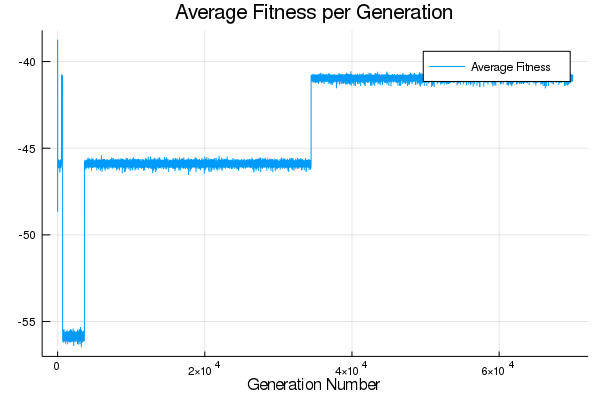
\includegraphics[scale=0.6]{average_fitness_per_generation.png}
    \caption{Average Fitness per Generation}
    \label{fig:avg_fitness_per_gen}
\end{figure}

\FloatBarrier{}
\section{Summary}

All three algorithms found an optimal solution to the problem. MIQP was the
fastest at $0.03$ seconds, BLP was the second fastest at $0.42$ seconds, at the
genetic algorithm was the slowest at $20.47$ seconds.

\FloatBarrier{}
\bibliography{citations}
\bibliographystyle{plain}

\end{document}
